\chapter{Research Philosophy and Overview}
\label{chap:research_overview}

This chapter presents the research philosophy that underpins the thesis and provides an overview of how its individual contributions are connected. Rather than considering the investigated technologies as isolated solutions, the thesis interprets them as successive methodological interventions along a broader progression from heterogeneous data towards actionable knowledge and AI-supported decision-making. This perspective, summarised in Figure~\ref{fig:research_perspective}, combines three complementary dimensions: (1) the Data--Information--Knowledge--Wisdom (DIKW) model~\cite{peters_dikw_2025}, adopted as a conceptual framework, describes the transformation through which diverse observations are progressively converted into information, knowledge, and ultimately actionable insights; (2) the data-centric methodology identifies the principal intervention points through which these transformations can be operationalised, namely \emph{Harmonization and Structuring}, \emph{Semantic Enrichment}, and \emph{Inference and Reasoning}; and (3) Trustworthy AI provides a cross-cutting perspective through which the resulting methods and systems can be interpreted. 
This conceptualisation provides the basis for organising the contributions presented in the following chapters.

\begin{figure}[t]
    \centering
    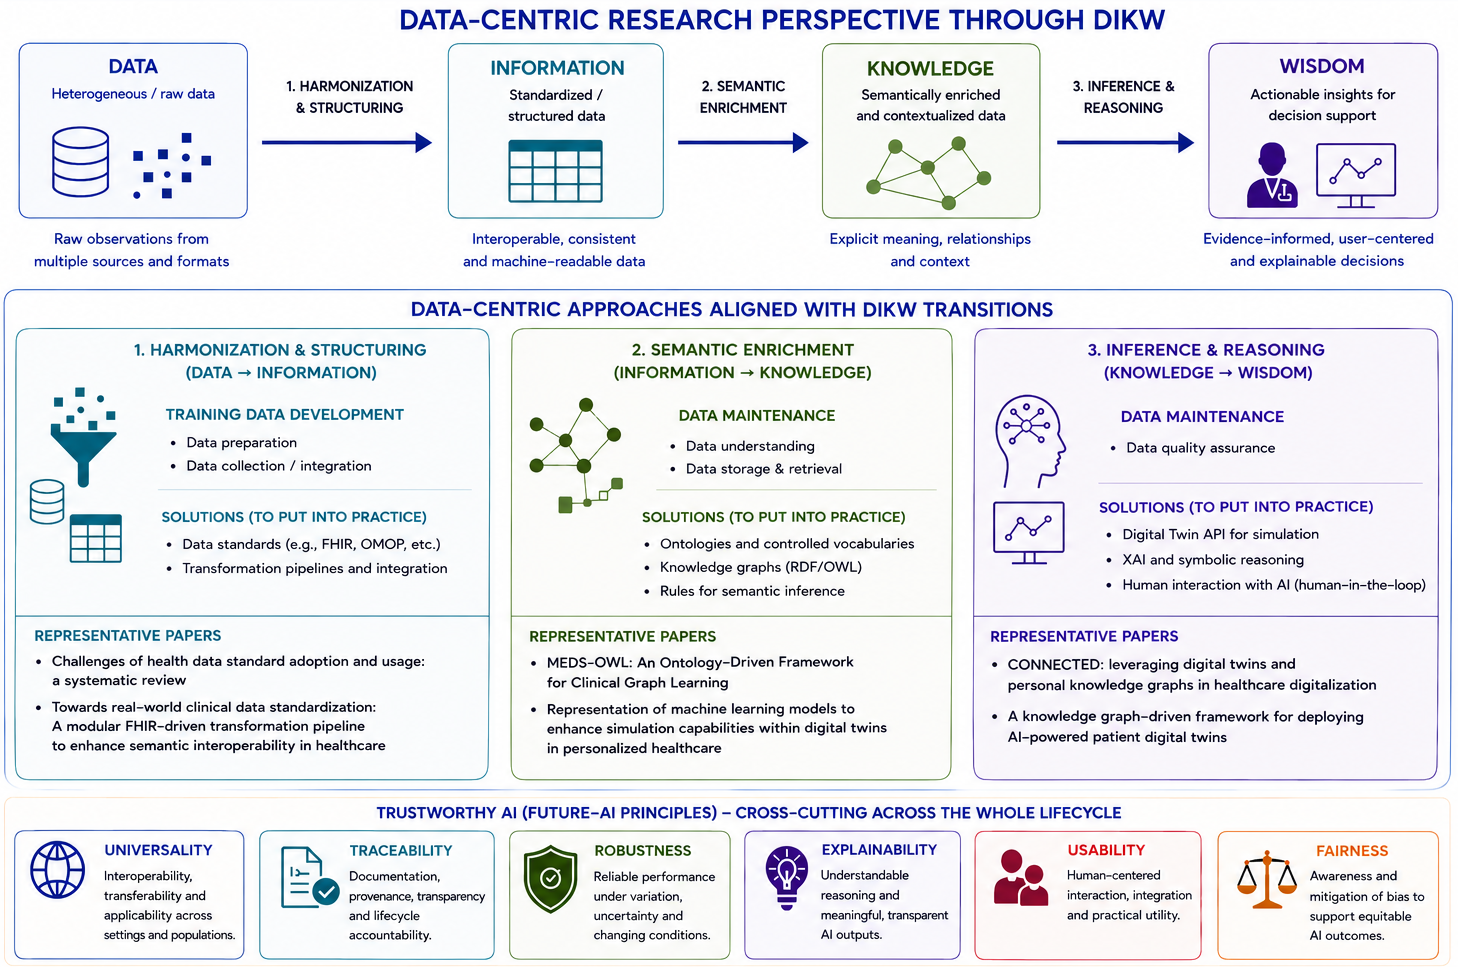
\includegraphics[width=\textwidth]{figures/fig1.png}
    \caption{Data-centric research perspective through the DIKW progression. The three methodological stages represent the principal transitions investigated in the thesis, while Trustworthy AI principles provide a cross-cutting perspective across the data and AI lifecycle.}
    \label{fig:research_perspective}
\end{figure}


\section{Research Methodology}
\label{sec:research_methodology}

The thesis adopts a data-centric perspective to investigate how heterogeneous data can be progressively transformed into knowledge and ultimately support AI-enabled decision-making. Three complementary dimensions provide the conceptual and methodological foundation of this work.

First, the thesis adopts the DIKW model as a conceptual lens for structuring its research trajectory. Its conventional linear interpretation has been criticised for overlooking the roles of context, experience, human judgement, and social factors in the formation of knowledge and wisdom~\cite{peters_dikw_2025}. Accordingly, DIKW is not treated here as a strict or deterministic hierarchy, nor is its final stage understood as an attempt to computationally reproduce human wisdom. Rather, it provides a conceptual framework for characterising the successive transformations examined across the thesis and for situating its research contributions within a common conceptual trajectory. Within this interpretation, the four levels represent progressively richer forms of representation and use. \emph{Data} refers to heterogeneous observations originating from different sources. \emph{Information} refers to data that have been organised and harmonised into a structured representation. \emph{Knowledge} adds explicit semantics, relationships, and contextual information. Finally, \emph{Wisdom} is operationalised in this thesis as the application of knowledge and inference to derive actionable insights that can support informed and human-centred decision-making.

\begin{equation}
\label{eq:DIKW}
\textbf{Data}
\xrightarrow{\text{(a)}}
\textbf{Information}
\xrightarrow{\text{(b)}}
\textbf{Knowledge}
\xrightarrow{\text{(c)}}
\textbf{Wisdom}
\end{equation}

Second, the progression \ref{eq:DIKW} is operationalised through three methodological stages: (a) \emph{Harmonization and Structuring} addresses the transition from heterogeneous data to structured and interoperable information, (b) \emph{Semantic Enrichment} introduces explicit semantics and relationships to transform information into machine-interpretable knowledge, and (c) \emph{Inference and Reasoning} exploits the resulting knowledge to support AI-driven analysis, simulation, and decision-making. These stages therefore represent the principal data-centric intervention points investigated by the thesis, rather than rigidly sequential processing steps.

Third, the principles of Trustworthy AI introduced in Chapter~\cref{chap:introduction} provide the ethical, technical, and societal foundation for the development and use of AI systems. In the healthcare domain, the FUTURE-AI framework~\cite{lekadir_future-ai_2025} provides a complementary practical perspective by translating these broad principles into concrete guidance for trustworthy healthcare AI. Initiated in 2021 by an international consortium of 117 researchers and healthcare professionals from 50 countries, FUTURE-AI defines six principles for trustworthy healthcare AI: \emph{Fairness, Universality, Traceability, Usability, Robustness}, and \emph{Explainability}. It further provides 30 best practices spanning the AI lifecycle, from design and development to validation, deployment, and monitoring~\cite{lekadir_future-ai_2025}. In this thesis, FUTURE-AI is therefore adopted as a cross-cutting framework, rather than as an additional stage in the proposed data-centric progression. Its principles are considered across the three methodological stages, with their relevance discussed in relation to the corresponding research contributions and the evidence provided by each contribution.

The three dimensions should not, however, be interpreted as strictly sequential or independent processing steps. Rather, they represent interconnected intervention points within a broader data and AI lifecycle. Data may be revisited as new requirements emerge. This iterative perspective reflects the broader data-centric view adopted by the thesis, in which the development of reliable AI systems requires continuous attention to data. %, their representation, their meaning, and their use.
This conceptualisation provides the organisational principle for the remainder of this chapter and for the presentation of the research contributions in the following chapters.

\section{Harmonization and Structuring}
\label{sec:harmonization_structuring}
The first stage is closely related to the \emph{Training Data Development} dimension of data-centric AI, which encompasses activities such as data collection, integration, and preparation. This transition transforms heterogeneous data into structured and interoperable information. This is particularly important in healthcare, where data are often fragmented across systems, limiting their availability and reuse for both primary and secondary purposes. Such fragmentation contributes to the persistent characterisation of health systems as \emph{health data rich and information poor}~\cite{murdoch_interpretable_2019}. The OECD similarly identifies weak data foundations and misaligned policies and practices as important barriers to the effective use of AI in healthcare~\cite{oecd_collective_2024,oecd_interoperability_2026}.

Interoperability is a central aspect in this context. It extends beyond the technical exchange of data to their consistent interpretation and use across systems and stakeholders. It encompasses different dimensions, including technical, semantic, organisational, and legal aspects~\cite{oecd_interoperability_2026}. At this stage, the focus is primarily on establishing compatible structures and representations that allow heterogeneous data to be consistently integrated and processed.

Accordingly, this stage establishes the intermediate data foundation required for subsequent transformations. By leveraging data standards and transformation pipelines, it produces structured and reusable information that can support subsequent semantic enrichment and inference.

\subsection{Background}
\label{subsec:harmonization_background}

Data standardisation provides one of the principal mechanisms through which this transition can be addressed~\cite{oecd_interoperability_2026}. It represents a key enabler of interoperability by providing common structures, representations, and conventions through which heterogeneous data can be exchanged and reused. For AI applications, these foundations are particularly important because standardised representations can facilitate data integration, improve consistency, and support the reproducibility and reuse of datasets across computational workflows~\cite{oecd_collective_2024}. Aligning standardisation practices with broader ethical and governance principles can further contribute to the development of Trustworthy AI in healthcare~\cite{srivastava_promoting_2023}. Consequently, the operationalisation of standards through data transformation processes represents an inherently data-centric approach to establishing the foundations for reliable AI systems.

\paragraph{Interoperability}

Interoperability can be understood as the ability of two or more systems or components to exchange information and to make effective use of the information exchanged~\cite{geraci1991ieee}. The concept, however, extends beyond the purely technical exchange of data and encompasses different dimensions of interaction. In this regard, the European Commission's National Interoperability Framework Observatory (NIFO) identifies four complementary dimensions of interoperability: \emph{legal}, \emph{organisational}, \emph{semantic}, and \emph{technical}.

The value of interoperability extends beyond technical efficiency. OECD estimates suggest that effective interoperability could generate benefits equivalent to 2.7\%--6.6\% of annual health expenditure~\cite{oecd_interoperability_2026}. Conversely, the costs of poor interoperability are significant: diagnostic errors account for an estimated 17.5\% of healthcare costs, while 81.5\% of physicians consider inadequate interoperability a potential risk to patient safety~\cite{oecd_interoperability_2026}. By enabling data to be accessed and interpreted consistently across systems, interoperability therefore provides an important foundation for the development and reuse of high-quality datasets for AI applications. Achieving effective interoperability requires the adoption of data standards~\cite{oecd_interoperability_2026}; however, standardisation is not a one-size-fits-all exercise, as different standards address different aspects and purposes within the health data ecosystem.

\paragraph{Data Standards}

As reported by a recent OECD study~\cite{oecd_interoperability_2026}, many countries are pursuing the harmonisation of health data and processes through the adoption of data standards, with 41\% relying exclusively on international standards. The health data standards landscape is extensive and covers different functions, broadly including vocabulary, content, communication, privacy and security, and identifiers~\cite{oecd_interoperability_2026}. Consequently, the selection and implementation of standards should consider the entire data lifecycle, making standardisation an inherently data-centric approach.

Several standards address different aspects of the health information ecosystem. As illustrated in Figure~\ref{fig:health_data_standards}, terminologies such as SNOMED CT and ICD-10 support the representation of clinical concepts and classifications, while HL7 FHIR enables the exchange of healthcare information. Other standards address longitudinal record management, such as openEHR, or the organisation of observational data for secondary use, such as OMOP-CDM~\cite{oecd_interoperability_2026}. Their complementary roles highlight that interoperability depends not only on adopting standards, but also on selecting and applying them according to the intended use and position of data within the health information lifecycle.

\begin{figure}[t]
    \centering
    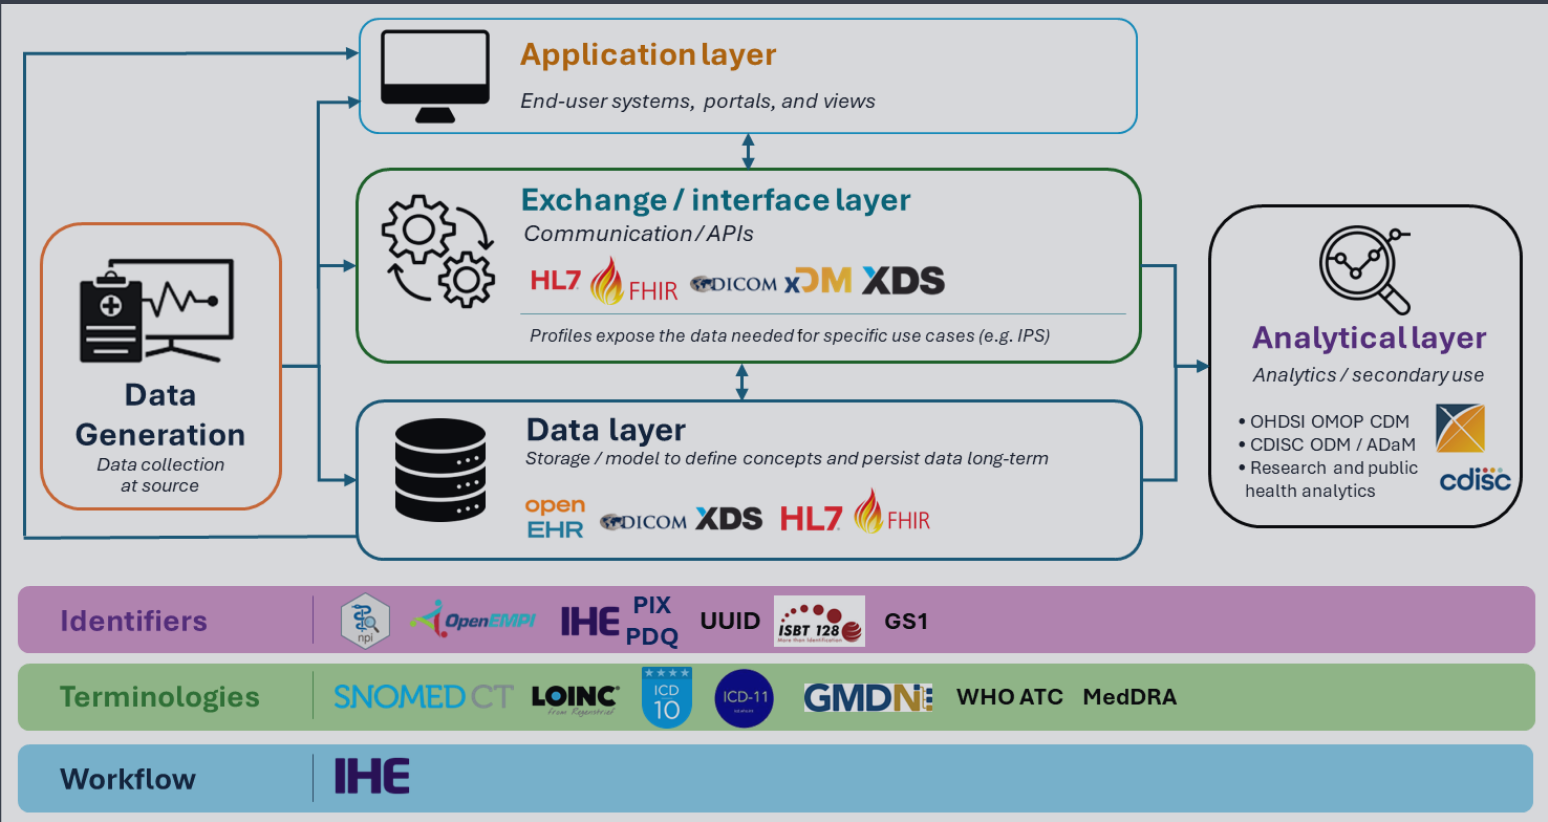
\includegraphics[width=\textwidth]{figures/fig2.png}
    \caption{Examples of available health data standards and their roles in interoperability. The figure is reproduced from~\cite{oecd_interoperability_2026}; the standards shown are illustrative and not prescriptive for all use cases.}
    \label{fig:health_data_standards}
\end{figure}

\paragraph{The European Health Data Space}

Regulatory frameworks and legislation are fundamental to successful interoperability efforts~\cite{oecd_interoperability_2026}. Beyond technical standards, effective health data sharing requires common rules governing access, exchange, and reuse. In Europe, the European Health Data Space (EHDS) represents a major initiative in this direction, establishing a common framework for the primary and secondary use of electronic health data across Member States~\cite{oecd_interoperability_2026}.

The EHDS brings together technical, organisational, and regulatory elements around a common goal: a patient-centred health data ecosystem in which data are findable, accessible, interoperable, and reusable (FAIR), and can be used effectively and safely in the public interest~\cite{oecd_interoperability_2026}. It aims to facilitate individuals' access to and control over their electronic health data across borders, while supporting their secure reuse for research, innovation, and data-driven policymaking.

By establishing common requirements for data access, interoperability, and reuse, the initiative seeks to address the fragmentation of health data across national and institutional systems~\cite{oecd_interoperability_2026}. This is particularly relevant for AI, which depends on sufficiently large, high-quality, and interoperable datasets for the development, validation, and deployment of models across different healthcare settings~\cite{oecd_progress_2026}.

\paragraph{Transformation pipelines}
The adoption of data standards requires practical mechanisms for transforming heterogeneous source data into standardised representations. Transformation pipelines operationalise this process through extraction, restructuring, mapping, and validation, supporting interoperability, secondary use, and the preparation of clinical data for analytics and AI~\cite{namli2024scalable,tabari2022state}. Existing approaches have demonstrated the feasibility of transforming heterogeneous clinical data into FHIR-based representations, including MIMIC-IV~\cite{bennett2023mimic}, openEHR compositions~\cite{ladas2022openehr}, and OMOP-CDM data~\cite{soares2023omop}, as well as through broader harmonisation and metadata-driven integration frameworks~\cite{williams2023standardized,simon2024metadata}. However, these approaches reveal recurring limitations concerning the portability and reusability of mapping processes, which may depend on internal mapping logic, custom scripts, implementation-specific technologies, or manual mapping and validation~\cite{bennett2023mimic,montazeri2023developing,sinaci2023data,williams2023standardized,ladas2022openehr,simon2024metadata}. Declarative and templated mappings can reduce some of these dependencies, although their applicability may remain constrained by specific mapping languages or input models~\cite{sinaci2023data,williams2023standardized,soares2023omop}. More recent work has explored modular FHIR- and RDF-based pipelines for producing research-ready and semantically enriched datasets, while highlighting the need for broader validation and further automation~\cite{carbonaro2025raw}. These limitations motivate transformation mechanisms that provide standardised and shareable mappings while reducing dependence on custom scripts and implementation-specific technologies.

\subsection{Contributions}
\label{subsec:harmonization_contributions}
The contributions associated with the first methodological stage address the transition from heterogeneous data to structured and interoperable information. Within the data-centric perspective adopted by this thesis, this transition is addressed through \emph{Harmonization and Structuring}, where data standards and transformation mechanisms provide the means to establish a common representation across heterogeneous sources. The two contributions investigate complementary aspects of this problem. The first characterises the current landscape of health data standard adoption and identifies the practical challenges that limit the effective use of standards. The second builds on these observations by investigating how standard-based transformation can be operationalised through a modular and reusable pipeline.

%$\paragraph{Characterising the adoption of health data standards.}
\paragraph{Paper 1 – health data standard adoption.}
The first contribution, \emph{Challenges of health data standard adoption and usage: a systematic review}~\cite{marfoglia2026challenges}, investigates how three major health data standards, FHIR, OMOP-CDM, and openEHR, are adopted and used in real-world clinical and research settings. The systematic review analyses 99 studies published between 2021 and 2024, considering their application domains, use cases, implementation scale, standard coverage, ETL approaches, and the extent to which the standards were adopted as specified or adapted to individual contexts.

The contribution provides an empirical characterisation of the conditions under which health data standards are adopted and implemented. In particular, it highlights the heterogeneity of existing practices and shows that the availability of a standard does not, by itself, ensure its consistent adoption or the harmonisation of heterogeneous data. The findings therefore identify a gap between the conceptual availability of standardised representations and their practical realisation in data transformation processes.

From the perspective of the thesis, this contribution constitutes the \emph{problem-characterisation} component of the Data--Information transition. It establishes that interoperability cannot be reduced to selecting a standard; it also requires appropriate processes for mapping, transforming, validating, and maintaining data across heterogeneous source environments.

%\paragraph{Operationalising standard-based data transformation.}
\paragraph{Paper 2 – standard-based data transformation.}
Building on this problem characterisation, the second contribution, \emph{Towards real-world clinical data standardization: A modular FHIR-driven transformation pipeline to enhance semantic interoperability in healthcare}~\cite{marfoglia_towards_2025}, investigates how the transformation of heterogeneous clinical data into a common standardised representation can be operationalised. The proposed approach combines a templating strategy with the FHIR Mapping Language and separates mapping specifications from their execution. The resulting pipeline adopts a modular architecture organised into five modules: \emph{Input}, \emph{Refinement}, \emph{Mapping}, \emph{Validation}, and \emph{Export}.

The approach was evaluated using real-world clinical data, transforming 1,962 hospital-stay records corresponding to 1,006 patients into 15 types of FHIR resources. The evaluation demonstrates the feasibility of applying the proposed transformation strategy to heterogeneous clinical data while preserving the information required by the target representation.

Within the thesis methodology, this contribution therefore represents the \emph{technical operationalisation} of the Data--Information transition. While the systematic review identifies the practical challenges associated with the adoption of health data standards, the transformation pipeline investigates how these challenges can be addressed through an explicit, modular, and reusable transformation process. The two contributions consequently form a progression from \emph{understanding the problem} to \emph{engineering a mechanism for addressing it}.

\paragraph{Overall contribution.}
Taken together, these contributions establish the foundation for the subsequent stages of the thesis and address complementary activities within the \emph{Training Data Development} dimension of data-centric AI~\cite{zha_data-centric_2025}. The FHIR-based clinical data collection study~\cite{arcobelli2024fhir,marfoglia2025towards} provides an example of \emph{Data Collection}, demonstrating how a common standard can be used to structure clinical information at the point of acquisition. The systematic review~\cite{marfoglia2026challenges} identifies the challenges associated with the practical adoption of health data standards, thereby providing an understanding of the current standardisation landscape upon which the FHIR transformation pipeline~\cite{marfoglia2025towards} builds. The latter operationalises \emph{Data Integration} and \emph{Data Preparation} through an explicit, modular, and reusable transformation process. Collectively, these contributions illustrate how data-centric principles can be translated into complementary mechanisms for collecting, understanding, harmonising, and preparing heterogeneous data for subsequent computational use.

These mechanisms also have direct relevance to Trustworthy AI. In particular, they provide evidence relevant to the FUTURE-AI principle of \emph{Universality}~\cite{lekadir_future-ai_2025}, encompassing interoperability, applicability, adaptability, and generalisability. Standardised representations and reusable transformation mechanisms facilitate the exchange and reuse of data across heterogeneous systems and contexts. The explicit definition of transformation rules and the modular separation of mapping specifications from their execution additionally provide elements relevant to \emph{Traceability}~\cite{lekadir_future-ai_2025}, as the transformation process can be made explicit and reproducible. Together, these properties promote greater transparency and control in the preparation of data for downstream processing.

\section{Semantic Enrichment}
\label{sec:semantic_enrichment}

The second methodological stage addresses the transition from \emph{Information} to \emph{Knowledge}. While harmonization and structuring establish compatible representations for heterogeneous data, standardization alone does not necessarily make their meaning, relationships, and contextual dependencies explicit. This stage therefore extends the data-centric process through semantic technologies that represent domain concepts and relationships in a machine-interpretable form.

It is primarily related to the \emph{Data Maintenance} dimension of data-centric AI, particularly \emph{data understanding} and \emph{data storage and retrieval}~\cite{zha_data-centric_2025}. Within the perspective adopted by this thesis, these activities are extended through formal semantic representations that make domain concepts, relationships, and contextual dependencies explicit and computationally accessible. Semantic Web technologies, ontologies, knowledge graphs, and semantic reasoning provide complementary mechanisms for enriching structured information and establishing a computable knowledge layer. This layer can subsequently support both AI methods and reasoning over interconnected information.

\subsection{Background}
\label{subsec:semantic_background}

\paragraph{Semantic Web.}

The Semantic Web (SW) provides formal mechanisms for representing information and its relationships in a machine-interpretable form~\cite{rathee_semantic_2025}. Among its core technologies, the Resource Description Framework (RDF) provides a graph-based data model for representing information as subject--predicate--object triples, while the Web Ontology Language (OWL) provides a formal language for defining concepts, properties, relationships, and logical constraints~\cite{amato_semfedxai_2025,xhani_role_2025}. Together, these technologies support graph-based representations in which heterogeneous resources can be explicitly connected and queried according to their semantic relationships~\cite{rathee_semantic_2025}.

This capability is particularly relevant to healthcare, where information originates from heterogeneous sources and is expressed using different structures and terminologies. By linking data to external terminologies, ontologies, and controlled vocabularies, Semantic Web technologies associate observations with explicit domain concepts and relationships, supporting data exploration, integration, and validation~\cite{toure2023}. Their extensibility also facilitates the integration of additional resources without requiring the underlying representation to be redesigned~\cite{rathee_semantic_2025}.

From a data-centric perspective, semantic technologies therefore extend data engineering beyond structural consistency by explicitly representing the meaning associated with data. They can also support the implementation of FAIR principles by facilitating semantic interoperability, structured access, knowledge integration, and data validation, although FAIRness ultimately depends on appropriate data governance and stewardship in addition to technological mechanisms~\cite{rathee_semantic_2025}. The role of semantic technologies in this thesis is consequently not limited to enriching datasets with additional metadata, but to establishing representations in which domain meaning can be computationally accessed and exploited.

\paragraph{Ontologies.}

Ontologies provide formal representations of the concepts, properties, and relationships that characterise a domain. By making domain semantics explicit, they establish a shared conceptual basis for interpreting and integrating heterogeneous data~\cite{xhani_role_2025,amato_semfedxai_2025}. In healthcare, resources such as SNOMED CT, LOINC, and ICD-10 illustrate the role of formalised vocabularies in representing clinical and biomedical concepts~\cite{amato_semfedxai_2025}.

By associating data elements with explicit domain concepts and relationships, ontologies support \emph{data understanding} and can reduce ambiguity arising from heterogeneous representations. They can also provide a semantic interface between data and AI methods by linking model features, predictions, or explanations to domain concepts. For example, medical ontologies have been used to enrich XAI outputs with clinically relevant contextual knowledge~\cite{corbucci_semantic_2023}, while DoctorXAI links features from sequential clinical data to ontology concepts to generate semantically meaningful explanations~\cite{panigutti_role_2023}.

In this sense, ontologies can complement XAI methods by providing the domain concepts and relationships through which AI outputs can be interpreted, although semantic representations alone do not guarantee explainability~\cite{xhani_role_2025}. Rather, they provide a structured semantic basis upon which explanation mechanisms can be constructed and contextualised.

\paragraph{Knowledge Graphs.}

Knowledge Graphs (KGs) represent interconnected entities and relationships in a graph-based structure. In Semantic Web applications, they are commonly represented using RDF and can be associated with ontologies that provide the conceptual semantics of the represented entities and relations~\cite{xhani_role_2025}. In this setting, ontologies provide the conceptual semantics used to describe a domain, while knowledge graphs instantiate such semantics through concrete entities, facts, and relationships.

This combination facilitates the integration of heterogeneous information while supporting semantic querying, provenance representation, and reasoning over interconnected data~\cite{xhani_role_2025}. It is particularly relevant to healthcare, where clinically meaningful information involves relationships among patients, observations, diagnoses, medications, procedures, and temporal events. Healthcare KGs have consequently been investigated for applications including diagnosis, drug-interaction detection, and personalised treatment~\cite{amato_semfedxai_2025}.

The resulting graph structure can also be exploited directly by AI methods. Graph-based learning approaches operate on entities and relations, while neuro-symbolic approaches combine learned representations with structured knowledge and formal reasoning~\cite{garcez_neurosymbolic_2023,yang_give_2024}. KGs therefore provide not only an alternative representation of data, but also a structured substrate through which semantic knowledge can be integrated with computational models.

 Once knowledge crystallises in the form of semantic graphs, it can be used to nurture and enhance AIs. The complexity of clinical data demands the use of intelligent systems that can reason over both explicit content and the nuanced context behind it. Knowledge graphs, for this purpose, have emerged as a powerful tool to build knowledge-enriched Artificial Intelligence systems. Information is structured to preserve its rich semantics and remains machine-interpretable, which enables AI systems to achieve context-aware understanding and inference instead of limiting themselves to surface-level pattern recognition \cite{maree_quantifying_2025}.


\paragraph{Semantic Inference and Reasoning.}

Explicit semantic representations can further support the derivation of knowledge that is not directly encoded in the original data. Ontologies provide the conceptual structures and logical constraints for representing domain knowledge, while rule-based formalisms such as the Semantic Web Rule Language (SWRL) enable additional facts to be inferred from explicitly represented information.

This capability has been explored to combine machine learning with explicit domain reasoning in healthcare-oriented AI systems~\cite{sharma_ontoxai_2024}. More broadly, neuro-symbolic approaches combine the representation and reasoning capabilities of symbolic systems with the predictive capabilities of neural networks~\cite{garcez_neurosymbolic_2023,bhuyan_neuro-symbolic_2024,yang_give_2024}. Recent approaches have also investigated the transformation of learned neural behaviour into symbolic rules or knowledge representations, making aspects of model behaviour more explicit and amenable to reasoning~\cite{terziyan_semantic_2026}. For example, OntoXAI uses SWRL-based representations to generate explanations from classification rules, while other neural-symbolic approaches integrate deep learning with ontologies and knowledge graphs to align learned representations with structured knowledge and support reasoning across heterogeneous information sources~\cite{cheng_neural-symbolic_2024}.

Overall, semantic representations provide the formal basis for making domain knowledge explicit and computationally accessible. The resulting knowledge can then be queried, integrated, and subjected to logical or computational inference. Within the data-centric perspective of this thesis, these mechanisms therefore provide the means through which structured information can be transformed into a machine-interpretable knowledge layer. Their subsequent exploitation for prediction, simulation, and decision support is considered in the \emph{Inference and Reasoning} stage.

\subsection{Contributions}
\label{subsec:semantic_contributions}

The contributions associated with the second methodological stage address the transition from structured \emph{Information} to machine-interpretable \emph{Knowledge}. Building on the standardised representations established in the previous stage, they investigate how semantic models can make both clinical data and computational resources explicitly representable and exploitable by AI systems. The two contributions address complementary aspects of this problem: the first focuses on the semantic representation of clinical event data and its integration with graph-based learning, while the second extends semantic representation to machine-learning models for personalised healthcare.

\paragraph{Paper 3 -- semantic representation of clinical data.}

The third contribution, \emph{MEDS-OWL: An Ontology-Driven Framework for Clinical Outcome Prediction with Graph Learning}, investigates how an event-centric representation of longitudinal clinical data can be transformed into a semantically explicit knowledge representation suitable for both data integration and graph-based learning. The work builds on the Medical Event Data Standard (MEDS), which provides a unified event-centric representation designed to support reproducible machine-learning workflows, but does not natively provide an ontology-level semantic representation. The contribution addresses this gap through \emph{MEDS-OWL}, a lightweight OWL ontology for MEDS, and \emph{meds2rdf}, a scalable framework for transforming MEDS-compliant datasets into RDF-based knowledge graphs.

The resulting representation preserves the event-centric structure of MEDS while introducing explicit semantics and relationships among subjects, events, and clinical concepts. The framework also enables links to external biomedical vocabularies, providing a basis for semantic integration and further enrichment of the generated knowledge graphs. The work therefore extends a standardised machine-learning-oriented data representation with an explicit semantic layer without requiring changes to the underlying MEDS model.

The contribution further investigates the role of semantic representation in AI by systematically varying the granularity of the relationships encoded in the resulting knowledge graphs. The framework was evaluated on four heterogeneous clinical datasets, comprising more than 309,000 hospital stays, and the resulting representations were used in 11 clinical outcome prediction tasks based on a Relational Graph Convolutional Network. The results show that increasing semantic granularity consistently improved Macro-F1 across the evaluated tasks, demonstrating that the choice of semantic representation can influence not only interoperability and knowledge representation but also the computational exploitation of clinical data through graph-based learning.

Within the thesis methodology, this contribution therefore represents the \emph{semantic operationalisation} of the Information--Knowledge transition. It extends the harmonised representation established in the previous stage by introducing explicit meaning and relationships, while simultaneously demonstrating that these representational choices influence how the resulting knowledge can be exploited by AI methods.

\paragraph{Paper 4 -- semantic representation of ML models.}

The fourth contribution, \emph{Representation of ML Models to Enhance Simulation Capabilities Within Digital Twins in Personalized Healthcare}, extends semantic representation beyond clinical data to the computational capabilities that operate on them. The work builds on the CONNECTED framework, which integrates heterogeneous healthcare data, FHIR-compliant representations, Personal Knowledge Graphs, and Digital Twins to support patient-specific services and predictive simulation.

The contribution introduces the \emph{Model Interface Manifest Ontology (MIMO)}, an OWL ontology developed in Protégé to formally describe executable ML models through their inputs, outputs, metadata, and location. These descriptions are represented as RDF and integrated with the semantic resources of the Digital Twin. Together with RDF-based patient data, an OWL Description Logic reasoner is then used to infer correspondences between model input requirements and available FHIR data, enabling the automatic invocation of models when the required inputs are satisfied~\cite{marfoglia_2024_mimo}.

Within the thesis methodology, this contribution extends the Information--Knowledge transition from the representation of clinical information to the representation of \emph{computational capabilities}. While MEDS-OWL makes clinical entities and their relationships explicit, MIMO makes the interfaces and metadata of AI models explicit, allowing data and computational resources to be connected within a common semantic environment. This representation makes computational capabilities identifiable and machine-interpretable, providing a semantic basis for their automated discovery, integration, and orchestration within an AI-enabled Digital Twin.

\paragraph{Overall contribution.}

Taken together, these contributions extend the data-centric perspective from the preparation of structured information to its maintenance, interpretation, and accessibility through explicit semantic representations. They operationalise aspects of the \emph{Data Maintenance} dimension by addressing complementary activities related to \emph{Data Understanding} and \emph{Data Storage and Retrieval}~\cite{zha_data-centric_2025}. Data understanding is addressed through the formalisation of the meaning and relationships of clinical information, while storage and retrieval are extended through semantic representations that make clinical data and computational resources identifiable, queryable, and reusable.

From the perspective of the thesis, \emph{Semantic Enrichment} therefore operationalises Data Maintenance by transforming structured information into a semantically organised and reusable knowledge space. The resulting computable knowledge layer provides a common environment in which clinical entities, relationships, and computational capabilities can be explicitly represented and connected. This establishes the basis for the subsequent \emph{Inference and Reasoning} stage, where the resulting knowledge and computational capabilities can be exploited for prediction, simulation, and decision support.

The semantic layer also provides technical foundations relevant to Trustworthy AI and, in particular, to the FUTURE-AI principles of \emph{Universality}, \emph{Traceability}, and \emph{Explainability}~\cite{lekadir_future-ai_2025}. By explicitly representing clinical concepts, relationships, and model interfaces, the proposed approaches facilitate the integration and reuse of information across heterogeneous environments while making relevant data and computational dependencies more explicit and inspectable. These properties can support the development of AI systems whose data and computational dependencies are more transparent and can provide semantic foundations for explanation mechanisms. However, they should be regarded as enabling mechanisms rather than evidence of full compliance with FUTURE-AI, which also requires broader validation, governance, and human-centred practices across the AI lifecycle.

\section{Inference and Reasoning}
\label{sec:inference_reasoning}

The third methodological stage addresses the transition from \emph{Knowledge} to actionable insights that can support informed and human-centred decision-making. While semantic enrichment establishes explicit and machine-interpretable representations of domain knowledge, this stage concerns the exploitation of such knowledge through inference, prediction, simulation, and AI-supported analysis. The objective is therefore not simply to represent information more richly, but to create an environment in which data, semantic knowledge, and computational capabilities can be combined to derive and evaluate context-dependent insights.

Within the data-centric perspective adopted by this thesis, this stage is primarily related to \emph{Data Maintenance}, particularly \emph{data quality assurance}~\cite{zha_data-centric_2025}. Data quality is not a property that can be established once and then considered permanent. In operational AI systems, data sources, patient states, computational environments, and intended uses may evolve over time, requiring continuous assessment of the information provided to AI methods and of the conditions under which their outputs are generated~\cite{zha_data-centric_2025}. In this context, inference and reasoning extend the data-centric perspective from the preparation and representation of data towards their use in dynamic computational environments. Digital Twins provide an architectural environment for integrating data, knowledge, and computational models, while explainability and human-in-the-loop mechanisms support the interpretation, assessment, and appropriate use of the resulting outputs.

\subsection{Background}
\label{subsec:inference_background}

\paragraph{Digital Twins.}

Digital Twins (DTs) have traditionally been used to represent, monitor, and simulate physical entities and processes across different application domains. In healthcare, they have emerged as an enabling technology for Healthcare 4.0, supporting applications such as patient monitoring, personalised treatment planning, clinical process optimisation, and simulation~\cite{9255249_erol,9900390_alazab,Björnsson2019,Katsoulakis2024}. Their applications span different levels of abstraction, including human- and organ-level modelling, treatment and drug-interaction simulation, remote healthcare, hospital resource management, medical-device monitoring, and the representation of healthcare processes and workflows~\cite{SHENGLI2021100014,Björnsson2019,9325551_ricci,8846667_yang_peng,9320532_elayan_haya}. In particular, Human Digital Twins aim to integrate heterogeneous biological, genetic, lifestyle, and clinical information to support the evaluation of possible interventions and future health states in a virtual environment~\cite{SHENGLI2021100014,Björnsson2019}.

The increasing availability of heterogeneous and continuously generated data has progressively expanded the role of DTs beyond static representation and simulation. More recent approaches conceptualise DTs as information-rich computational environments in which heterogeneous data, semantic representations, and computational models are integrated to support monitoring, analysis, prediction, and simulation~\cite{felicetti_knowledge_2025,Katsoulakis2024}. Within such architectures, ontologies can provide a semantic foundation for representing domain concepts and relationships, while knowledge graphs support the integration of heterogeneous entities and contextual information~\cite{boje_towards_2020,albers_semantic_2020}. AI methods can then operate on this structured environment to identify patterns, generate predictions, and support simulation and decision-making~\cite{felicetti_knowledge_2025}. This evolution changes the role of the Digital Twin within the overall data-centric process. Rather than representing a physical or clinical entity in isolation, the DT can act as an integration layer connecting the different elements required for computational analysis.

Such an environment is particularly relevant to personalised healthcare, where patient-specific information can be combined with predictive models and simulation mechanisms to investigate possible trajectories or interventions~\cite{Katsoulakis2024}. At the same time, the increasing complexity of these environments introduces additional requirements concerning data quality, semantic consistency, privacy and security, and the validation and appropriate use of computational models~\cite{Katsoulakis2024}. Consequently, the reliability of a healthcare DT depends not only on the predictive capabilities of its constituent models, but also on the quality and contextual validity of the data, knowledge, and computational relationships supporting them.

\paragraph{Human-in-the-Loop and XAI.}

The exploitation of AI-generated knowledge in healthcare also requires mechanisms through which computational outputs can be interpreted, assessed, and appropriately incorporated into human decision-making. Human-in-the-loop approaches therefore maintain human involvement in relevant stages of the AI workflow, including the interpretation of outputs, validation of system behaviour, and assessment of AI-supported decisions~\cite{kaur_trustworthy_2022,felicetti_knowledge_2025}. Human involvement is particularly important in healthcare because computational outputs are ultimately interpreted within clinical and organisational contexts that cannot be reduced to the information available to an individual model.

Explainable AI (XAI) provides a complementary set of mechanisms for supporting this interaction by making aspects of model behaviour or individual predictions more understandable to human stakeholders~\cite{guidotti_survey_2019,miller_explanation_2019}. Depending on the application and intended user, explanations may concern individual predictions or provide more general information about model behaviour~\cite{murdoch_interpretable_2019,xhani_role_2025,kaur_trustworthy_2022}. They can support activities such as model inspection, debugging, identification of potentially problematic behaviour, and feature analysis~\cite{10.1145/2939672.2939778_ribeiro}. However, the adequacy of an explanation depends on its intended purpose, scope, and audience, particularly in healthcare where explanations must be meaningful within the relevant clinical context~\cite{kaur_trustworthy_2022}.

The need for such mechanisms becomes more pronounced as Digital Twins evolve towards adaptive systems that combine heterogeneous data, semantic knowledge, and AI models for prediction and simulation~\cite{felicetti_knowledge_2025}. Machine-learning models can identify complex statistical patterns, but their outputs do not necessarily expose the domain knowledge or contextual relationships underlying those patterns~\cite{felicetti_knowledge_2025}. Semantic technologies can complement this capability by providing an explicit contextual layer through which data, concepts, relationships, and computational resources can be connected~\cite{boje_towards_2020,albers_semantic_2020}. Ontologies and knowledge graphs can consequently support the interpretation of model inputs and outputs by relating them to domain concepts and contextual information~\cite{xhani_role_2025}, while expert-curated semantic structures can provide additional constraints for reducing unsupported interpretations or inferences~\cite{karabulut_ontologies_2024}.

Within this perspective, semantic representation and explainability address complementary aspects of human understanding. XAI provides mechanisms for exposing relevant aspects of model behaviour, whereas semantic representations provide the domain context through which computational outputs can be related to concepts, entities, and relationships~\cite{xhani_role_2025,corbucci_semantic_2023,panigutti_role_2023}. Their combination can therefore support a workflow in which human stakeholders receive computationally derived insights, relate them to the underlying patient and domain context, and assess their relevance before incorporating them into decision-making~\cite{felicetti_knowledge_2025}. Importantly, neither semantic representation nor explanation alone guarantees correctness, reliability, or appropriate use. Rather, they provide technical mechanisms that can support human understanding and oversight within a broader trustworthy AI lifecycle.

\subsection{Contributions}
\label{subsec:inference_contributions}

The contributions associated with the third methodological stage investigate how semantically enriched \emph{Knowledge} can be exploited to support AI-enabled analysis in the form of \emph{Wisdom}. This stage focuses on computational environments where patient information can be leveraged by AI to predict possible trajectories and support personalised medicine.

The two contributions follow a progressive trajectory. The first introduces the architectural foundations for integrating heterogeneous and standardised patient data within a Digital Twin\cite{10.3389/fdgth.2023.1322428_carbonaro_connected}. The second extends this virtual replica with simulation capabilities~\cite{MARFOGLIA2026108380}. It hides the underlying technical complexity behind an effective interface that can be directly exploited by stakeholders. The resulting environment exposes semantically enriched and contextualised outputs, facilitating their interpretation and assessment by human users.

\paragraph{Paper 5 - Digital Twins and Personal Knowledge Graphs.}
The first contribution, \emph{CONNECTED: leveraging digital twins and personal knowledge graphs in healthcare digitalization}~\cite{10.3389/fdgth.2023.1322428_carbonaro_connected}, investigates how Digital Twins and Knowledge Graphs can provide an architectural foundation for integrating heterogeneous healthcare data and supporting intelligent applications. The gathered and harmonized data are used to populate patient-specific Digital Twins. The resulting virtual replicas provide a persistent representation of patient information and establish the basis for analytical and simulation capabilities.

This contribution extends data quality considerations beyond the initial preparation of a dataset. Patient-specific representations depend on the availability and evolution of their underlying data sources. The information supporting downstream computational processes must therefore remain structured, coherent, and up to date. The Digital Twin provides an environment in which patient data can be maintained and interpreted within their computational context. It thus connects data quality assurance with the subsequent use of data for AI-enabled analysis and decision support.

\paragraph{Paper 6 -- AI-powered patient Digital Twins.}
The second contribution, \emph{A knowledge graph-driven framework for deploying AI-powered patient digital twins}~\cite{MARFOGLIA2026108380}, extends CONNECTED towards the integration and operational use of AI models within the Digital Twin. It enables the virtual replica to dynamically connect patient-specific information with computational models and support predictive simulation.

A key contribution is the automation of model integration. The framework abstracts the underlying technical complexity through an API, allowing stakeholders to focus on insight-driven applications. The benchmarking experiment demonstrates this capability by integrating and continuously evaluating multiple AI models within the same environment. Beyond model comparison, it shows how the Digital Twin can act as a dynamic and semantically harmonised repository of patient-specific information. This capability is relevant to the data-centric perspective because it brings data quality into the model lifecycle. It also facilitates human oversight within a common computational environment.

\paragraph{Overall contribution.}
Taken together, these contributions address the transition from \emph{Knowledge} to actionable insights. They combine semantically enriched patient information with AI models and simulation capabilities. CONNECTED provides the architectural foundation for integrating heterogeneous and standardised patient data within a Digital Twin backed by a Knowledge Graph. The subsequent framework extends this foundation towards the operational integration of AI models and predictive simulation.

From a data-centric perspective, this stage extends \emph{Data Maintenance}, particularly \emph{data quality assurance}, into the operational use of AI systems~\cite{zha_data-centric_2025}. Patient data, semantic representations, and AI models are maintained within a common computational environment, allowing data quality and contextual validity to remain connected to downstream inference. The Digital Twin therefore acts as an integration layer between the \emph{Knowledge} established in the previous stage and its computational exploitation.

The resulting approach also provides elements relevant to Trustworthy AI and human-in-the-loop decision-making. The explicit representation of patient information, semantic relationships, and computational capabilities supports \emph{Traceability}, while the integration of AI capabilities through higher-level interfaces facilitates their use by human stakeholders~\cite{lekadir_future-ai_2025}. More broadly, combining semantic context, predictive models, and human interaction provides enabling mechanisms for \emph{Usability}, \emph{Robustness}, and \emph{Explainability}, supporting the interpretation and assessment of AI-generated insights rather than replacing human judgement~\cite{lekadir_future-ai_2025}.
